% Template for Cogsci submission with R Markdown

% Stuff changed from original Markdown PLOS Template
\documentclass[10pt, letterpaper]{article}

\usepackage{cogsci}
\usepackage{pslatex}
\usepackage{float}
\usepackage{caption}

% amsmath package, useful for mathematical formulas
\usepackage{amsmath}

% amssymb package, useful for mathematical symbols
\usepackage{amssymb}

% hyperref package, useful for hyperlinks
\usepackage{hyperref}

% graphicx package, useful for including eps and pdf graphics
% include graphics with the command \includegraphics
\usepackage{graphicx}

% Sweave(-like)
\usepackage{fancyvrb}
\DefineVerbatimEnvironment{Sinput}{Verbatim}{fontshape=sl}
\DefineVerbatimEnvironment{Soutput}{Verbatim}{}
\DefineVerbatimEnvironment{Scode}{Verbatim}{fontshape=sl}
\newenvironment{Schunk}{}{}
\DefineVerbatimEnvironment{Code}{Verbatim}{}
\DefineVerbatimEnvironment{CodeInput}{Verbatim}{fontshape=sl}
\DefineVerbatimEnvironment{CodeOutput}{Verbatim}{}
\newenvironment{CodeChunk}{}{}

% cite package, to clean up citations in the main text. Do not remove.
\usepackage{apacite}

% KM added 1/4/18 to allow control of blind submission


\usepackage{color}

% Use doublespacing - comment out for single spacing
%\usepackage{setspace}
%\doublespacing


% % Text layout
% \topmargin 0.0cm
% \oddsidemargin 0.5cm
% \evensidemargin 0.5cm
% \textwidth 16cm
% \textheight 21cm

\title{Finding Common Ground: Referential communication in parent-child pairs}


\author{{\large \bf Morton Ann Gernsbacher (MAG@Macc.Wisc.Edu)} \\ Department of Psychology, 1202 W. Johnson Street \\ Madison, WI 53706 USA \AND {\large \bf Sharon J.~Derry (SDJ@Macc.Wisc.Edu)} \\ Department of Educational Psychology, 1025 W. Johnson Street \\ Madison, WI 53706 USA}

\begin{document}

\maketitle

\begin{abstract}
Include no author information in the initial submission, to facilitate
blind review. The abstract should be one paragraph, indented 1/8 inch on
both sides, in 9\textasciitilde{}point font with single spacing. The
heading `Abstract' should be 10\textasciitilde{}point, bold, centered,
with one line of space below it. This one-paragraph abstract section is
required only for standard six page proceedings papers. Following the
abstract should be a blank line, followed by the header `Keywords' and a
list of descriptive keywords separated by semicolons, all in
9\textasciitilde{}point font, as shown below.

\textbf{Keywords:}
referential pacts; parent-child communication
\end{abstract}

\hypertarget{introduction}{%
\section{Introduction}\label{introduction}}

As social beings, humans communicate with each other constantly. We use
words and gestures to convey different messages, but communication
relies on more than just the ability to speak or gesture---it requires
mutual understanding. Conversational partners must take into account
each other's knowledge and adjust their speech accordingly. For example,
adults talk to young children with simpler words and sentence structures
than when conversing with fellow adults. This sensitivity to other
people allows us to achieve mutual understanding, or common ground, with
our conversational partners. While research shows that adults readily
form common ground with one another (Brennan \& Clark, 1996; Clark \&
Wilkes-Gibbs, 1986), studies with children have yielded mixed results
(Branigan, Bell, \& McLean, 2016; Glucksberg \& Krauss, 1967). Children
eventually become skilled conversationalists, but little is known about
how they acquire and refine their communicative skills. The present
study focuses on referential communication between children and
caregivers, to further understand how children develop communicative
abilities, and the role that parents play in scaffolding this
development.

\hypertarget{conceptual-pacts}{%
\subsection{Conceptual Pacts}\label{conceptual-pacts}}

Providing sufficient information is essential to successful
communication (Grice, 1975), and doing so often requires reasoning about
other people's knowledge. For example, adults can use canonical labels
to refer to most objects, but may need to provide further information
when speaking with children, who have less vocabulary knowledge.
Linguists have found that successful communication relies on common
ground---shared knowledge that is constructed and modified in verbal
communication. Common ground ensures that conversational partners have
some mutual understanding upon which their communication can be based
on. In referential communication, which may center around referents that
are not immediately present, common ground can be particularly
important. Referential communication patterns in adults have been widely
studied, mostly using matcher-director paradigms. In these paradigms,
participants are paired up and asked to talk about abstract shapes or
pictures. The goal of the game is for the director to guide the matcher
to select a particular picture solely via verbal communication. These
studies capture how common ground is shaped between two conversational
partners. Clark and Wilkes-Gibbs (1986) found that common ground can be
established using conceptual pacts, which are agreed-upon terms or
phrases used to describe a particular referent. The researchers also
found a pattern of conceptual pact formation. Over a few rounds of the
game, utterances became shorter and more certain, and conversational
partners eventually converged upon a name for each abstract shape. It is
important to note that different conceptual pacts were formed for each
pair of participants. That is, common ground is more than common
sense---it is mutual knowledge that is built between partners within a
conversation.

Conceptual pacts are partner-specific, but malleable, and facilitates
cooperation between conversational partners. The formation of conceptual
pacts is collaborative and partner-specific, such that interlocuters
mutually come to agreement (whether explicitly or implicitly) about
these pacts, and continue to reuse them with one another, but not
necessarily with new partners (Brennan \& Clark (1996); Clark \&
Schaefer (1989)). At the same time, the mutual knowledge between
partners is temporary and fluid---it can be changed even within the span
of a single conversation, based on shifting goals or informational needs
(Ibarra \& Tanenhaus (2016)). Conceptual pact formation is not only a
natural process that occurs in conversation, it is also beneficial for
partners completing cooperative tasks (Fusaroli et al., 2012). These
studies, along with many others in the field, show that adults readily
form conceptual pacts with one another in conversation, and that these
pacts can facilitate cooperation.

Similar matcher-director studies have been conducted in children, but
have yielded mixed results. An early study by Glucksberg and Krauss
(1967) found that young children were unable to form common ground with
each other in a matcher-director task, even though they were able to
complete the task when familiar pictures were used. Although young
children may struggle to negotiate conceptual pacts with peers, they do
expect speakers to be referentially consistent, just like older children
and adults (Graham, Sedivy, \& Khu, 2014). Other studies have shown that
children are able to form referential pacts with others by the age of 6,
and by age 10, are sensitive to multiple partners' knowledge states
(Branigan et al., 2016; Köymen, Schmerse, Lieven, \& Tomasello, 2014).
Taken together, these studies suggest that children's ability to
reliably form conceptual pacts with one another emerge in early
childhood, and continue to develop through middle childhood.

Thus far, research on children's communicative development have largely
focused on peer interactions. While these studies allow us to see how
children's referential abilities differ at various ages, they may not
capture the full picture. Children do not only interact with each other.
Indeed, much of young children's daily interactions involve adults such
as caregivers and teachers. To better understand how children become
skilled conversationalists, we must explore the role that adults play in
children's communicative development.

\hypertarget{parent-child-interaction}{%
\subsection{Parent-Child Interaction}\label{parent-child-interaction}}

Young children interact with their caregivers on a daily basis. Research
in the field of language development has found that linguistic input
from parents and caregivers are predictive of children's language
learning outcomes (Weisleder \& Fernald, 2013). While many studies have
examined how parental speech influences children's acquisition of
vocabulary and grammar, less research has been done on how parents
scaffold children's communicative development more broadly. Language
learning does not occur in isolation, and a broader understanding of
language development requires that we study that communicative contexts
in which language is used. Parents and caregivers are sensitive to their
children's needs, and are able to adapt their language accordingly. When
interacting with young children, parents modify their sentence structure
and content based on their children's vocabulary knowledge (Leung,
Tunkel, \& Yurovsky, in press; Masur, 1997). In an observational study
by Masur (1997), parents and children played with toy animals. The
author found that parents used different sentence structures when
referring to animals, depending on whether their children were familiar
with the animal's canonical label. In a more recent study, Leung et
al.~(in press) examined parents' speech in a communicative game, where
parents guided children to select animals on an iPad screen. Results
showed that parents used longer sentences with more adjectives when
referring to animals that they believe their children do not know. Taken
together, these studies show that parents are able to sensitively adapt
their language based on their children's developmental level. How might
conversing with more linguistically-advanced interlocuters influence
children's communicative development? There is some evidence that adults
can scaffold children's referential communication (Glucksberg \& Krauss,
1967; Matthews, Lieven, \& Tomasello, 2010). As mentioned above,
preschoolers were unable to complete the matcher-director task with
peers in Glucksberg \& Krauss' (1967) study. However, in a follow up
study, experimenters asked preschoolers to name the abstract objects
prior to playing the game. When an adult experimenter used the
preschoolers' preferred referent names, children were able to complete
the task. This finding suggests that children's failure to complete the
referential communication task may lie in their inability to negotiate
conceptual pacts with one another, rather than an inability to map a
referent name onto a referent.

Explicit feedback may also influence children's referential
communication abilities. Matthews et al.~(2010) conducted a training
study, in which young children received explicit feedback from adult
experimenters in a referential communication setting. Participants who
underwent training were more likely to spontaneously produce unambiguous
referential expressions at test, indicating that feedback can support
the development of communicative abilities. However, both studies
discussed here examine adult-child interaction in a highly constrained
setting: the adults are experimenters with a clear script of how to
speak to the child participants. To better understand how adults may
scaffold children's communicative development, we must study adult-child
interactions in a more naturalistic setting.

The present study aims to explore how parents and children interact to
form referential pacts in conversation. Based on prior developmental
research showing that sensitivity to conceptual pacts emerge in early
childhood, and referential abilities gradually develop through middle
childhood (Branigan et al., 2016; Graham et al., 2014; Köymen et al.,
2014), we opted to study 4-8 year-old children. This study was intended
to be largely exploratory, with no particular a priori hypotheses about
the results. The main goal of this is to understand whether and how
parents scaffold children's communicative development, by comparing
parent-child referential communication across ages.

\hypertarget{experiment-1-parent-child-interaction}{%
\section{Experiment 1: Parent-Child
Interaction}\label{experiment-1-parent-child-interaction}}

\hypertarget{methods}{%
\subsection{Methods}\label{methods}}

\begin{CodeChunk}
\begin{figure*}[h]

{\centering 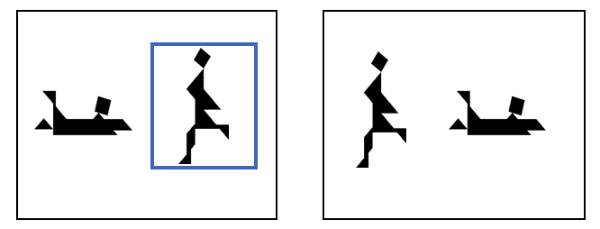
\includegraphics{figs/2-col-image-1} 

}

\caption[Example of iPad screens for the director (left) and matcher (right) during the game]{Example of iPad screens for the director (left) and matcher (right) during the game.}\label{fig:2-col-image}
\end{figure*}
\end{CodeChunk}

\hypertarget{participants}{%
\subsubsection{Participants}\label{participants}}

Children (ages 4, 6, and 8) and their parents were recruited from a
database of families in the local community, to achieve a planned sample
of 60 parent-child pairs. A total of 75 children and their parents
participated, but data from 12 pairs were dropped due to experimental
error or failure to complete the study. The remaining sample of 63
parent-child dyads were included in analysis.

\hypertarget{stimuli}{%
\subsubsection{Stimuli}\label{stimuli}}

Twelve solid black images of tangrams, and colored versions of the same
tangrams, were selected from a database of Public Domain images. The
tangram images were normed on Amazon Mechanical Turk (mTurk) for
pairwise similarity. Two images were excluded from the set based on
similarity judgments, forming the final set of 10 images used for the
study.

\hypertarget{procedure}{%
\subsubsection{Procedure}\label{procedure}}

Each parent-child pair played a cooperative game with iPads. Pairs sat
at a table with a divider in the middle, which prevented parents and
children from looking at each other's iPad screens during the game. The
game was a simplified version of the matcher-director task used in Clark
\& Wilkes-Gibbs (1986). Parents and children were told that they would
take turns being the director and matcher. They were told that the
director should describe the image inside the blue square, and the
matcher should select an image based on the director's description.
After instruction, the practice and experimental trials began. On each
experimental trial, two solid black tangrams appeared on the iPad
screens. The same images appeared on each screen, but their positions
were randomized. On the director's screen, one image appeared inside a
blue square, while the images on the matcher's screen simply appeared on
a white background (Figure 1). Upon selection of an image on the
matcher's screen, the selected image became colorful, and a sound is
played (independent of accuracy). After each trial, the roles were
switched. Practice trials followed the same structure as experimental
trials, but images of fruits and vegetables were used during this round.
All sessions were videotaped. All videos were transcribed using an
Open-Source coding software, Datavyu (2014).

\hypertarget{design}{%
\subsubsection{Design}\label{design}}

There were 4 blocks of 10 trials. Each tangram appeared as the target
once during each block, such that each tangram was the target four times
during the game. Trials within blocks were randomized. The 10 tangrams
were shuffled and randomly assigned to either the parent or the child at
the beginning of the game. The assignment dictates who would be the
director for a particular trial in Round 1. Thus, parents and children
played the role of director two times for each of the 10 tangrams. In
each round, the targets appeared with different foils. To ensure that
the task would not be too difficult for young children, the trials were
constructed such that the most similar tangrams (based on mTurk worker
judgments) did not appear together.

\hypertarget{results}{%
\subsection{Results}\label{results}}

\hypertarget{reduction-in-length-of-referring-expression}{%
\subsubsection{Reduction in length of referring
expression}\label{reduction-in-length-of-referring-expression}}

\begin{CodeChunk}
\begin{figure}[b]

{\centering 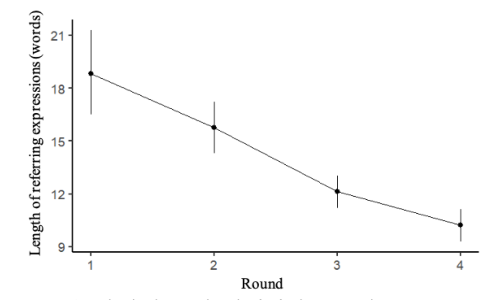
\includegraphics{figs/reduction-1} 

}

\caption[Reduction in mean length of referring expressions across four rounds]{Reduction in mean length of referring expressions across four rounds.}\label{fig:reduction}
\end{figure}
\end{CodeChunk}

\begin{CodeChunk}
\begin{figure}[h]

{\centering 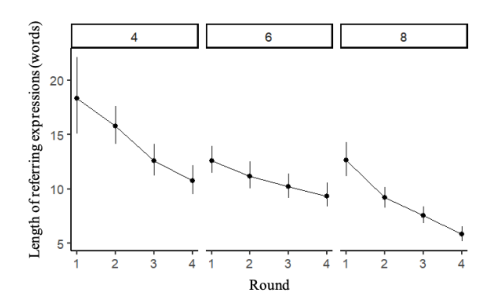
\includegraphics{figs/development-1} 

}

\caption[Change in length of referring expressions, split by age groups]{Change in length of referring expressions, split by age groups.}\label{fig:development}
\end{figure}
\end{CodeChunk}

We began our analyses by calculating mean length of referring
expressions for each target, and examining change in length across
rounds. Only the directors' speech was included in this calculation.
Collapsing across parents and children, and all age groups, the length
of referring expressions decreased somewhat linearly from Round 1 to
Round 4 (Figure 2). When splitting by age group, analyses revealed that
dyads with older children used shorter referring expressions overall,
while the main effect of length reduction held across groups (Figure 3).
The difference in length of referring expressions was particularly clear
between 4-year-olds and 8-year-olds, with 6-year-olds falling somewhat
in between the two groups.

We then analyzed parents and children's referring expressions
separately. When splitting parents and children, and plotting by age
groups, we still found an overall reduction in length of referring
expression (Figure 4). However, when looking only at children's
referring expressions, the three groups did not appear to differ. On the
other hand, the three groups of parents differed in their length of
referring expressions. Specifically, parents of 4-year-olds used longer
referring expressions throughout the game. Note that only 2 rounds are
plotted in this figure, because each partner is the director twice for
each target tangram.

\hypertarget{reaction-time}{%
\subsubsection{Reaction Time}\label{reaction-time}}

We analyzed reaction time for each trial. Reaction time was stored
automatically by the game's computer code, and can be understood as time
taken to complete the trial (rather than reaction time to a stimulus per
se). Reaction times longer than 20000ms (2 minutes) were discarded.
Since the game did not have an option for pausing, trials had abnormally
long reaction times when dyads needed to take a break from the game
(e.g.~children needing to use the bathroom). Similar to length of
referring expressions, reaction time decreased from Round 1 to Round 4
for pairs in all age groups (Figure 5). When split by age group,
reaction times showed similar patterns to length of referring
expression, such that dyads with older children were faster overall
(Figure 6).

\hypertarget{discussion}{%
\section{Discussion}\label{discussion}}

Our main effect of reduction in length of referring expression
replicates the effect found in Clark and Wilkes-Gibbs (1986), suggesting
that parents and children were forming conceptual pacts with one another
as the game progressed (Figure 2). This effect was found across all
three age groups, and patterns were largely similar across groups. Our
results show that children as young as 4 are able to cooperate with a
more linguistically capable partner to form conceptual pacts in
conversation. Taken together with prior research suggesting that
4-year-olds are not yet able to form conceptual pacts with their peers
(Glucksberg \& Krauss, 1967), our findings indicate that adults could
scaffold younger children's conversational abilities to facilitate
effective referential communication.

Older children and their parents used shorter referring expressions
overall (Figure 3). This finding may reflect older children's more
advanced linguistic skills compared to their younger counterparts, such
that they produce more succinct (and perhaps more efficient) referring
expressions. Older children may also require less descriptive
information about the target tangram in order to identify it. These
explanations are not mutually exclusive, but further analysis suggests
that the latter may reflect our data more accurately.

When analyzing length of referring expression separately for parents and
children, we found that the age difference was largely driven by parents
(Figure 4). While children's length of referring expression did decrease
across rounds, patterns did not seem to differ across age groups. On the
other hand, parents of 4-year-olds used longer referring expressions
than parents of older children. One potential reason for why parents
used longer referring expressions with younger children could be that
these children required more scaffolding. Younger children may have
difficulty focusing on relevant dimensions of the target tangram, such
that parents need to provide more information in order for their
children to select the correct tangram. Qualitative analysis is
currently underway, and will be helpful for understanding the reason
parents use varying lengths of referring expressions with their
children. Our analyses thus far suggest that parents may be adapting
their speech for effective communication, using longer, more informative
sentences with younger children, and shorter ones with older children.

Reaction times decreased across rounds for all parent-child pairs
(Figure 6). Our reaction time analyses showed patterns similar to that
of length of referring expressions. While dyads across age groups showed
the same pattern of decreasing reaction time, older children and their
parents were faster overall. These results show that parents and
children are calibrated to each other during the game. If reaction times
did not match length of referring expressions, that could indicate that
parents and children were providing too little or too much information
to each other, such that the two measures would be mismatched. Thus, the
intuitive finding that reaction times matched referring expression
lengths serves to strengthen the argument that parents calibrate to
their children in communicative settings.

Thus far, our analyses show that children can cooperate with their
parents to form conceptual pacts about novel referents. Given that
children as young as 4 years old were successful in forming referential
pacts with others, our results suggest that parents, who are more
linguistically-advanced, can scaffold children's communicative
abilities. Qualitative analysis is currently ongoing, and will be
helpful for answering the following questions: How do parents and
children each drive the referential pact formation process? How do these
roles change across development? A deeper understanding of the
characteristics of parent-child referential communication across
development will shed light onto the how children develop their
conversational skills, and how parents may scaffold the process.

\hypertarget{future-directions}{%
\subsection{Future Directions}\label{future-directions}}

Adult conceptual pact formation has been widely studied, and the effects
have been fairly robust. The present study rests upon the assumption
that adults readily form conceptual pacts with one another in
referential communication settings, but a direct comparison between
parent-child pairs and adult-adult pairs playing the same game may be
helpful. We are currently recruiting adult participants to play the same
communication game. Since our study uses a simplified version of Clark
and Wilkes-Gibbs' (1986) original paradigm, recruiting adult
participants would be helpful for understanding children's developmental
trajectory between ages 4 and 8. Our data would allow us to ask how
parent-child pairs differ from adult-adult pairs, both quantitatively
and qualitatively.

A useful follow-up would be to alter the trials, such that similar
tangrams are paired together. Currently, tangrams that are most
dissimilar to each other are paired, as a way to ensure that the game
would not be too difficult for young children. Anecdotally, however, the
researchers have noticed that older children occasionally comment on the
game being too easy. Other than increasing the difficulty of the game,
pairing similar tangrams also has the important benefit of allowing us
to understand how different pressures influence referential
communication and conceptual pact formation. The follow-up study could
be directly compared to the current study, and would allow us to further
explore how parents calibrate to their children in referential
communication settings.

\hypertarget{acknowledgements}{%
\section{Acknowledgements}\label{acknowledgements}}

Place acknowledgments (including funding information) in a section at
the end of the paper.

\hypertarget{references}{%
\section{References}\label{references}}

\setlength{\parindent}{-0.1in} 
\setlength{\leftskip}{0.125in}

\noindent

\hypertarget{refs}{}
\leavevmode\hypertarget{ref-Branigan2016Do}{}%
Branigan, H. P., Bell, J., \& McLean, J. F. (2016). Do you know what i
know? The impact of participant role in children's referential
communication. \emph{Frontiers in Psychology}, \emph{7}, 1--15.
\url{http://doi.org/10.3389/fpsyg.2016.00213}

\leavevmode\hypertarget{ref-Brennan1996Conceptual}{}%
Brennan, S. E., \& Clark, H. H. (1996). Conceptual pacts and lexical
choice in conversation. \emph{Journal of Experimental Psychology:
Learning Memory and Cognition}, \emph{22}(6), 1482--1493.
\url{http://doi.org/10.1037/0278-7393.22.6.1482}

\leavevmode\hypertarget{ref-Clark1989Contributing}{}%
Clark, H. H., \& Schaefer, E. F. (1989). Contributing to discourse.
\emph{Cognitive Science}, \emph{13}(2), 259--294.
\url{http://doi.org/10.1016/0364-0213(89)90008-6}

\leavevmode\hypertarget{ref-Clark1986Referring}{}%
Clark, H. H., \& Wilkes-Gibbs, D. (1986). Referring as a collaborative
process. \emph{Cognition}, \emph{22}, 1--39.

\leavevmode\hypertarget{ref-Glucksberg1967What}{}%
Glucksberg, S., \& Krauss, R. (1967). What do people say after they have
learned how to talk? Studies of the development of referential
communication. \emph{Merrill-Palmer Quarterly of Behavior and
Development}, \emph{13}(4), 309--316.

\leavevmode\hypertarget{ref-Ibarra2016flexibility}{}%
Ibarra, A., \& Tanenhaus, M. K. (2016). The flexibility of conceptual
pacts: Referring expressions dynamically shift to accommodate new
conceptualizations. \emph{Frontiers in Psychology}, \emph{7}.
\url{http://doi.org/10.3389/fpsyg.2016.00561}

\bibliographystyle{apacite}


\end{document}
